\documentclass[dvipdfm]{beamer}
\usepackage{pgffor}
\usepackage{stysty}

\usetheme{Rochester}

\newtheorem*{requirement}{要請}
\newtheorem*{them}{定理}
\newtheorem*{defn}{定義}
\newtheorem*{goal}{目標}
\newtheorem*{exmpl}{例}

\setbeamertemplate{footline}[frame number]
\AtBeginSection[]{
    \frame{\tableofcontents[currentsection, hideallsubsections]} %目次スライド
}

\title{トポロジカル秩序の分類に制限を与える禁止定理}
\author{低音}

\begin{document}

\begin{frame}
    \titlepage
\end{frame}

\begin{frame}{2025年物性若手夏の学校やります!!!}
    \begin{itemize}
        \item 全国の物性物理関連の大学院生が集結
        \item 4泊5日の集中合宿
        \item 講義・集中ゼミで最先端研究をキャッチアップ
        \item 学会形式で自分の研究を発表
    \end{itemize}
    若手研究者が研究の道を本格的に歩み始める第一歩になります!!!

    \textbf{\red{参加・斡旋・各種協賛お願いします!!!}}

    \textbf{\red{$\downarrow$個人協賛応募フォーム$\downarrow$}}(調整中)
    \begin{figure}
        \centering
        
\includegraphics[width=0.2\linewidth]{QR_736654.png}
    \end{figure}
\end{frame}

\begin{frame}{自己紹介: 低音}
    \begin{columns}
        \begin{column}{0.6\textwidth}
            \begin{itemize}
                \item 京大 基礎物理学研究所 M1
                \item 専門は凝縮系理論物理
                \item 登山・自転車が趣味
                \item note「ペンローズのグラフ記法」
                \item 第70回物性若手夏の学校 副代表
            \end{itemize}
        \end{column}
        \begin{column}{0.3\textwidth}
            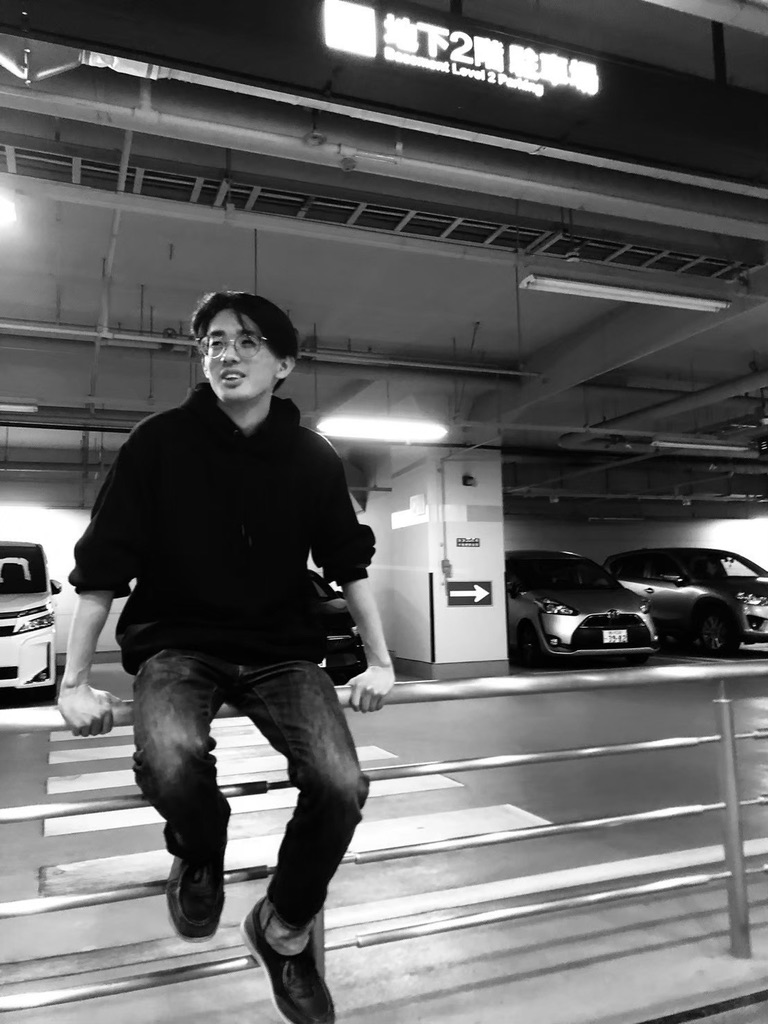
\includegraphics[width=1.2\linewidth]{38A299D4-7495-44B7-B699-E1AF92AFC245_1_105_c.jpeg}
        \end{column}
    \end{columns}
\end{frame}

\begin{frame}{このセミナーで目指すもの}
    \begin{goal}
        自発的対称性では説明できない相の分類を理解する
    \end{goal}
\end{frame}


\section{review: 自発的対称性の破れ}

\begin{frame}{理論と基底状態}
    \begin{defn}[固有方程式]
        \begin{equation*}
            \mqty[
                H_{11} & \cdots & H_{1N}
                \\
                \vdots & \ddots & \vdots
                \\
                H_{N1} & \cdots & H_{NN}
            ]
            \underset{\red{\text{固有状態ベクトル}}}{
                \mqty[
                    \phi_1 \\ \vdots \\ \phi_N
                ]
            }
            =
            \underset{\red{\text{固有値}}}{E}
            \underset{\red{\text{固有状態ベクトル}}}{
                \mqty[
                    \phi_1 \\ \vdots \\ \phi_N
                ]
            }
        \end{equation*}
        \begin{equation*}
            \hat{H}\ket{\phi}
            =
            E\ket{\phi}
        \end{equation*}
        \begin{equation*}
            \vcenter{\hbox{
                \begin{tikzpicture}
                    \node at(-1,0)[draw,rectangle](H){$H$};
                    \node at(0,0)[draw,rectangle](psi){$\ket{\phi}$};
                    \draw(H.east)--(psi.west)(H.west)--++(-.5,0);
                \end{tikzpicture}
            }}
            =
            E
            \vcenter{\hbox{
                \begin{tikzpicture}
                    \node at(0,0)[draw,rectangle](psi){$\ket{\phi}$};
                    \draw(psi.west)--++(-.5,0);
                \end{tikzpicture}
            }}
        \end{equation*}
    \end{defn}
    \begin{defn}[理論]
        エネルギーを固有値にもつ行列 $\hat{H}$
    \end{defn}
    \begin{defn}[基底状態]
        $\hat{H}$の最小固有値を出す固有状態。
        絶対零度では基底状態が実現する。
    \end{defn}
    \begin{defn}[\red{\textbf{状態の}}対称性]
        変換$\hat{U}$によって$\hat{U}\ket{\psi}\equiv\ket{\psi}$となること
    \end{defn}
    \begin{defn}[\red{\textbf{理論の}}対称性]
        変換$\hat{U}$によって$\hat{U}\hat{H}=\hat{H}\hat{U}$となること
    \end{defn}
\end{frame}

\begin{frame}{自発的対称性の破れ}
    \begin{defn}[自発的対称性の破れ (spontaneous symmetry breaking; SSB)]
        理論$\hat{H}$が対称性を持つが、系の基底状態がその対称性を持たないこと
    \end{defn}
    \begin{equation*}
        \vcenter{\hbox{
            \begin{tikzpicture}
                \draw[->, >=Stealth](-2,0)--(2,0)node[right]{$\ev{\hat{m}}$};
                \draw[->, >=Stealth](0,-.5)--(0,2)node[above]{$E=\ev{\hat{H}}$};
                \draw[domain=-1.75:1.75] plot(\x, {0.5*(\x-1)*(\x+1)*(\x-1)*(\x+1)-.5});
                \fill[red](1,-.5)circle(0.05)node[right]{実現する期待値};
            \end{tikzpicture}
        }}
    \end{equation*}
\end{frame}


\begin{frame}{自発的対称性の破れ}
    \begin{exmpl}[固体液体転移]
        \begin{itemize}
            \item 液体: 平行移動で対称
            \item 固体: 平行移動の対称性を\textbf{自発的に破る}
        \end{itemize}
        \begin{figure}
            \centering
            \begin{minipage}{0.45\linewidth}
                \centering
                \begin{tikzpicture}
                    \draw(0,0)rectangle(3,2);
                    \foreach\t in{0,1,...,100}{
                        \fill({mod(\t,11)*3/7},{mod(\t,7)*2/13})circle(.05);
                    }
                \end{tikzpicture}
            \end{minipage}
            \begin{minipage}{0.45\linewidth}
                \centering
                \begin{tikzpicture}
                    \draw(0,0)rectangle(3,2);
                \end{tikzpicture}
            \end{minipage}
        \end{figure}
    \end{exmpl}
\end{frame}


\begin{frame}{秩序変数と相の分類}
    \begin{defn}[秩序変数]
        自発的対称性の有無に応じて
        \begin{equation*}
            \ev{\hat{O}}{\mathrm{GS}}
            \begin{cases}
                =0 & (\text{sym. respect})
                \\
                \neq0 & (\text{sym. breaking})
            \end{cases}
        \end{equation*}
        となるような$\ev{\hat{O}}{\mathrm{GS}}$を秩序変数という。
    \end{defn}
    \begin{example}[固体液体転移]
    \end{example}
\end{frame}

\begin{frame}{Landau paradigm}
    相分類は自発的対称性の破れだけで決定できると思っていた。
    \begin{figure}
        \centering
        \begin{minipage}{0.45\linewidth}
            \centering
            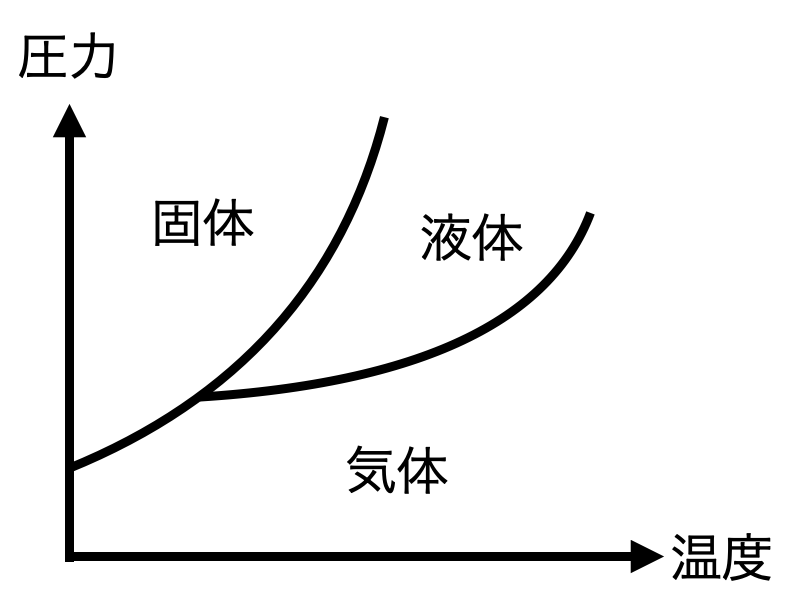
\includegraphics[width=0.8\linewidth]{phase3.png}
        \end{minipage}
        \begin{minipage}{0.45\linewidth}
            \centering
            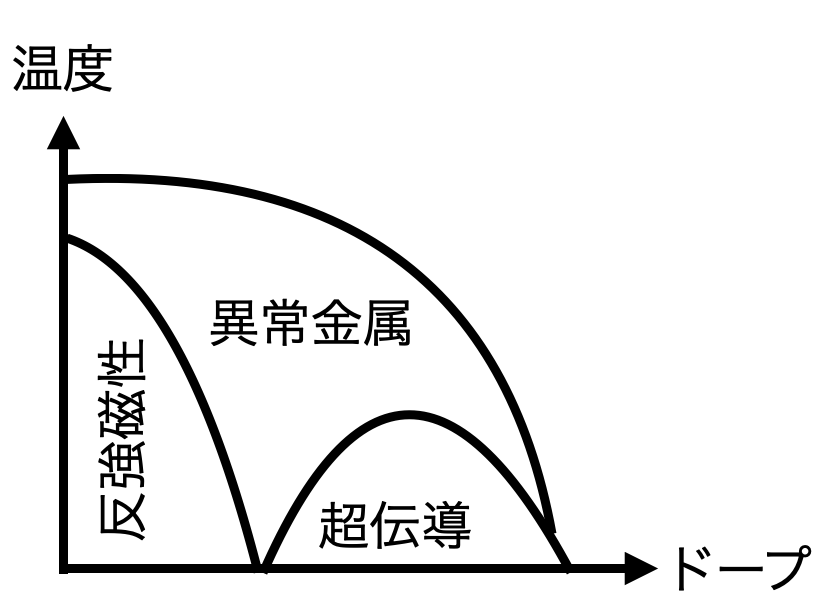
\includegraphics[width=0.8\linewidth]{phase-mag.png}
        \end{minipage}
    \end{figure}
    \begin{figure}
        \centering
        \begin{minipage}{0.45\linewidth}
            \centering
            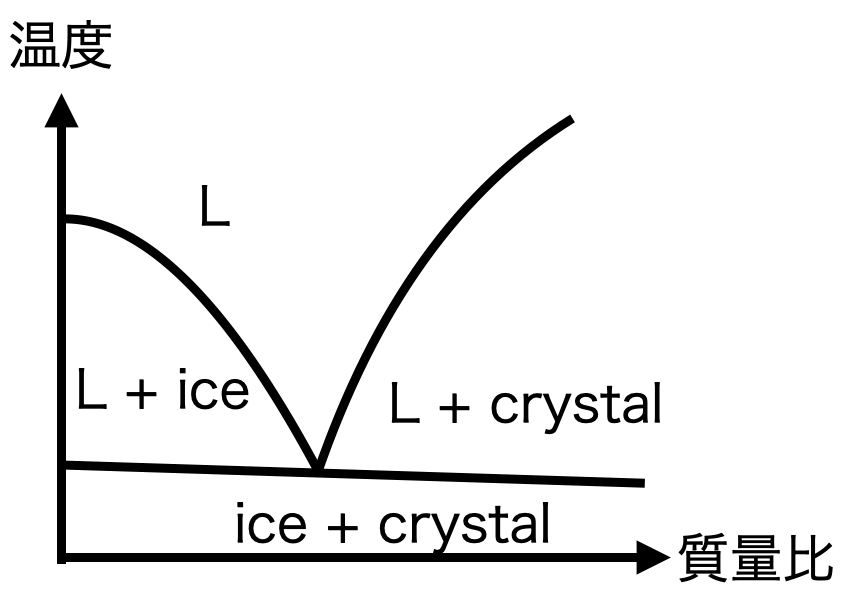
\includegraphics[width=0.8\linewidth]{melt.png}
        \end{minipage}
        \begin{minipage}{0.45\linewidth}
            \centering
            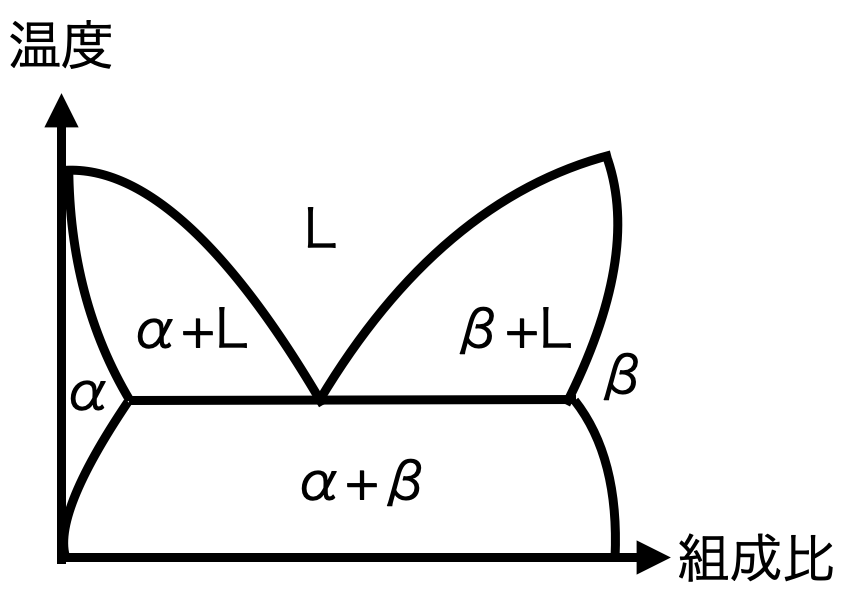
\includegraphics[width=0.8\linewidth]{solid2.png}
        \end{minipage}
    \end{figure}
\end{frame}


\section{beyond SSBの例: toric code}

\subsection{toric code}

\begin{frame}{toric code}
    トーラスに格子を張ってスピン1/2を配置.
    \begin{figure}
        \centering
        \includegraphics[width=0.4\linewidth]{./toric.pdf}
    \end{figure}
    \begin{equation*}
        \hat{H}
        =
        -J_e\sum_v\prod_{j: \text{link to }v}\sigma_j^x
        -J_m\sum_p\prod_{j: \partial p}\sigma_j^z
    \end{equation*}
    内部対称性は各方向$\pi$回転($\mathbb{Z}_2\times\mathbb{Z}_2$).
\end{frame}

\begin{frame}{toric codeのWilson line}{}
    灰色の線の周りを反転させる.
    \begin{figure}
        \centering
        \begin{tikzpicture}[scale=.8]
            % open line
            \fill[red, opacity=.1](1,0)rectangle(2,1);
            \fill[red, opacity=.1](4,1)rectangle(5,2);
            \draw[ultra thick, gray](1.5,.5)-|++(1,1)--++(2,0);
            % loop
            \draw[ultra thick, gray](0,-1.5)--++(6,0);
            \foreach\x in{0,1,...,5}{
                \draw(\x,-2)--++(0,4.5);
                \foreach\y in{-2,-1,0,1,2}{
                    \fill($(\x+.5,\y)$)circle(.1);
                    \fill($(\x,\y+.5)$)circle(.1);
                    \draw(\x,\y)--++(1,0);
                }
            }
            % open line
            \fill[red](1,.5)circle(.1);
            \fill[red](1.5,0)circle(.1);
            \fill[red](1.5,1)circle(.1);
            \draw(2,.5)circle(.15);
            \fill[red](2,1.5)circle(.1);
            \fill[red](2.5,0)circle(.1);
            \draw(2.5,1)circle(.15);
            \fill[red](2.5,2)circle(.1);
            \fill[red](3,.5)circle(.1);
            \draw(3,1.5)circle(.15);
            \fill[red](3.5,1)circle(.1);
            \fill[red](3.5,2)circle(.1);
            \draw(4,1.5)circle(.15);
            \fill[red](4.5,1)circle(.1);
            \fill[red](4.5,2)circle(.1);
            \fill[red](5,1.5)circle(.1);
            % loop
            \foreach\x in{0,1,...,5}{
                \fill[red]($(\x+.5,-1)$)circle(.1);
                \fill[red]($(\x+.5,-2)$)circle(.1);
                \draw(\x,-1.5)circle(.15);
            }
        \end{tikzpicture}
    \end{figure}
    線の端のplaquetteが励起.
    loopにすると励起が消滅する.
\end{frame}

\begin{frame}{toric codeの基底状態}{}
    トーラス$T^2$では\red{連続変形で移り変われないloop}の取り方が4種類.
    \begin{figure}
        \begin{tikzpicture}[scale=.5]
            \draw(0,0)circle(2 and 1);
            \draw(-1,0)arc(-120:-60:2);
            \draw(-.9,-.05)arc(120:60:1.8);
        \end{tikzpicture}
        \begin{tikzpicture}[scale=.5]
            \draw(0,0)circle(2 and 1);
            \draw(-1,0)arc(-120:-60:2);
            \draw(-.9,-.05)arc(120:60:1.8);
            \draw[gray, ultra thick](0,0)circle(1.5 and .7);
        \end{tikzpicture}
        \begin{tikzpicture}[scale=.5]
            \draw(0,0)circle(2 and 1);
            \draw(-1,0)arc(-120:-60:2);
            \draw(-.9,-.05)arc(120:60:1.8);
            \draw[gray, ultra thick](-2,0)arc(180:0:.5 and .4);
            \draw[gray, dashed, ultra thick](-2,0)arc(180:360:.5 and .4);
        \end{tikzpicture}
        \begin{tikzpicture}[scale=.5]
            \draw(0,0)circle(2 and 1);
            \draw(-1,0)arc(-120:-60:2);
            \draw(-.9,-.05)arc(120:60:1.8);
            \draw[gray, ultra thick](0,0)circle(1.5 and .7);
            \draw[gray, ultra thick](-2,0)arc(180:0:.5 and .4);
            \draw[gray, dashed, ultra thick](-2,0)arc(180:360:.5 and .4);
        \end{tikzpicture}
    \end{figure}
    loop $l_1, l_2$に沿って$\prod_{j\in l_i}\sigma_j^z$を取ると、それぞれ固有値が異なる。
    基底状態が直交して4重縮退.
    しかしいずれも\textbf{\alert{内部対称性を破っていない}}.
    \begin{equation*}
        \hat{U}\ket{\mathrm{GS}}
        =
        \ket{\mathrm{GS}}
        \qquad(\forall U\in\mathbb{Z}_2\times\mathbb{Z}_2)
    \end{equation*}
    \textbf{\alert{自発的対称性の破れだけでは相の分類が足りない?}}
\end{frame}


% \subsection{S=1 AF Heisenberg}


\section{量子相の分類問題}

\begin{frame}{量子相の分類}
    \begin{center}
        \includegraphics[width=\linewidth]{phase-diag.png}
    \end{center}
\end{frame}

\begin{frame}{エネルギーギャップ}
    \begin{example}[スピン1/2 Heisenbergモデル]
        \begin{equation*}
            H=-\sum_j\hat{\bm{S}}_j\cdot\hat{\bm{S}}_{j+1}
        \end{equation*}
        スピンが揃った状態が最安定だが、わずかに揺らせば実質エネルギー0で他の状態に移れる。
        \begin{figure}
            \centering
            \begin{tikzpicture}[xscale=3]
                \foreach\x in{0,0.1,...,1}{
                    \draw[->, >=Stealth]($(\x,0)+({-90+10*sin(\x*360)}:.5)$)--++({90-10*sin(\x*360)}:1);
                }
            \end{tikzpicture}
        \end{figure}
    \end{example}
    \alert{\red{$\rightarrow$外部からの擾乱に弱い}}
\end{frame}

\begin{frame}{エネルギーギャップ}
    \begin{figure}
        \centering
        \begin{minipage}{0.45\linewidth}
            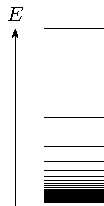
\includegraphics[width=0.3\linewidth]{gapless.pdf}
        \end{minipage}
        \begin{minipage}{0.45\linewidth}
            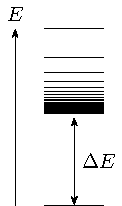
\includegraphics[width=0.3\linewidth]{gapped.pdf}
        \end{minipage}
    \end{figure}
    基底状態からのギャップが広ければ広いほど、外部からの擾乱で他の状態に変わりにくい。

    e.g. 量子ビットに最適!
\end{frame}

\begin{frame}{エンタングルメント (量子もつれ)}
    古典的確率で定式化できない相関
\end{frame}



\begin{frame}{量子相の分類・再掲}
    \begin{center}
        \includegraphics[width=\linewidth]{phase-diag.png}
    \end{center}
\end{frame}



% \begin{frame}{拡張されたLieb-Schultz-Mattis定理}
%     % $\hat{H}:=\sum_{x\in\Lambda}\hat{h}_x,\qquad|\mathrm{supp}\:\hat{h}_x|<R\ll L$に制限
%     \begin{them}[拡張Lieb-Schultz-Mattis定理]
%         基底状態がunique gappedのとき, 以下を満たす.
%         \begin{enumerate}
%             \item U(1)対称性, 並進対称性があるならフィリング$N/V$は整数.
%             \item 空間群$\mathcal{S}$, 有限可換群による内部対称性$G$, 全対称性$\mathcal{S}\times G$ならば2D系の格子ホモトピーが非自明.
%             \item 1D並進対称, on-siteの対称性が有限群ならば射影表現の乗数系が自明.
%             \item 1Dを1点で繋いだ空間$m$回回転対称, on-siteの対称性が有限群ならば中心点での対称性の乗数系$c_0\in H^2(G,U(1))$が$c_0=mc$と書ける.
%         \end{enumerate}
%     \end{them}
%     4つの条件のいずれかを破るとき, \textbf{\alert{基底状態が縮退 or gapless}}.
% \end{frame}

% \begin{frame}{拡張されたLieb-Schultz-Mattis定理}
%     \begin{figure}
%         \centering
%         \includegraphics[width=0.6\linewidth]{../img/phase-diag.png}
%     \end{figure}
%     \begin{exempli}
%         考えている系が
%         \begin{itemize}
%             \item 基底状態は対称性を破らない
%             \item ギャップあり
%             \item 前述の4つの条件のいずれかを破る
%         \end{itemize}
%         を全て満たすとき\alert{\textbf{基底状態がトポロジカルな縮退}}をすることが確実.
%     \end{exempli}

%     % \begin{eg}
%     %     \begin{itemize}
%     %         \item U(1), 並進対称非整数フィリングHubbard (縮退 or gapless)
%     %         \item toric code (基底状態が4重縮退)
%     %         \item スピン半奇数AF Heisenberg (gapless)
%     %     \end{itemize}
%     % \end{eg}

%     % 『ある条件』は満たさないとき, 確証はないが, 基底状態が非自明な量子相に属する可能性がある.
%     % (e.g. Haldane相)

%     % \begin{thm}[cf. U(1), 並進対象開放系]
%     %     並進対称性とstrong U(1)対称性のある開放系でfillingが非整数のとき, Lindbladianがgappedまたはsteady stateが縮退する.
%     % \end{thm}
% \end{frame}



% % % \section[]{ひねり境界条件による1次元半奇数Heisenbergモデルでの主張}

% % % \begin{frame}{1D半奇数AF Heisenbergモデル}
% % %     \begin{thm}[Lieb-Schultz-Mattis (1961), Affleck-Lieb (1986)]
% % %         1次元半奇数反強磁性Heisenbergモデル
% % %         \begin{equation*}
% % %             \hat{H}
% % %             =
% % %             \sum_{i}J\hat{\bm{S}}_i\cdot\hat{\bm{S}}_j
% % %             \qquad(J>0)
% % %         \end{equation*}
% % %         では, 熱力学極限で基底状態が縮退するかギャップレスになる.
% % %     \end{thm}

% % %     特にサイト数が偶数の有限系では基底状態がunique (Marshall-Lieb-Mattis theorem, \cite{Marshall1955} \cite{LiebMattis1962})であるため, 熱力学極限はギャップレスに限られる.
% % % \end{frame}


% % % \begin{frame}{証明方針}
% % %     長さ$L$周期境界条件で
% % %     \begin{table}
% % %         \begin{tabular}{ll}
% % %             捻り演算子 & $\hat{U}:=\exp(\sum_{x=1}^L2\pi ix/L)$
% % %             \\
% % %             基底状態 & $\ket{\mathrm{GS}}$
% % %             \\
% % %             試行状態 & $\hat{U}\ket{\mathrm{GS}}$
% % %         \end{tabular}
% % %     \end{table}
% % %     \begin{figure}
% % %         \centering
% % %         \includegraphics[width=0.5\linewidth]{../summer-school/img/torus-knot-straight.png}
% % %     \end{figure}
% % %     \begin{itemize}
% % %         \item $\ev{\hat{U}^{-1}\hat{H}\hat{U}}{\mathrm{GS}}=\order{L^{-1}}$: ギャップ無限小
% % %         \item $\ev{\hat{U}}{\mathrm{GS}}=\ev{\hat{T}^{-1}\hat{U}\hat{T}}{\mathrm{GS}}=0$: 低エネ状態が直交
% % %     \end{itemize}
% % %     \alert{熱力学極限スピン半奇数AF Heisenberg鎖では基底状態がunique gappedにならない!}
% % % \end{frame}


% % % \section[]{磁束の挿入によるU(1)対称な系のLSM定理 (case 1)}

% % % \begin{frame}{U(1)対称性でのLSM定理 (case 1)}
% % %     \begin{thm}[Lieb-Schultz-Mattis (1961), Oshikawa (2000), etc.]
% % %         \textbf{\alert{U(1)対称性}}と\textbf{\alert{並進対称性}}のある系で周期境界条件のもと, \textbf{\alert{単位格子あたりの粒子数(フィリング)が非整数}}なら\textbf{\alert{基底状態が縮退するかギャップレス}}になる.
% % %     \end{thm}

% % %     \begin{eg*}{}{}
% % %         非整数フィリング並進対称Hubbardモデルは縮退 or gapless:
% % %         \begin{equation*}
% % %             \hat{H}
% % %             =
% % %             \sum_{j\in\mathbb{Z}}
% % %             \sum_{\sigma=\uparrow,\downarrow}
% % %             tc_{j,\sigma}^\dag c_{j+1,\sigma}
% % %             +
% % %             (\mathrm{h.c.})
% % %             +
% % %             \sum_{j\in\mathbb{Z}}
% % %             Un_{j,\uparrow}n_{j,\downarrow}
% % %         \end{equation*}
% % %         次元を追加して周期境界条件と直行する向きにhoppingを加えても縮退 or gaplessのまま.
% % %     \end{eg*}
% % % \end{frame}

% % % \begin{frame}{定理の証明方針: 磁束の挿入 (case 1)}
% % %     粒子数$N$をfix.
% % %     \begin{minipage}{0.6\linewidth}
% % %         \begin{equation*}
% % %             \begin{split}
% % %                 \hat{H}_0
% % %                 & \quad \overset{\text{磁束量子の挿入}}{\longrightarrow} \quad
% % %                 \hat{H}_{2\pi}=\hat{U}\hat{H}_0\hat{U}^{-1}
% % %                 \\
% % %                 \ket{\mathrm{GS}_0}
% % %                 & \quad \overset{\text{磁束量子の挿入}}{\longrightarrow} \quad
% % %                 \ket{\mathrm{GS}_{2\pi}}
% % %             \end{split}
% % %         \end{equation*}
% % %     \end{minipage}
% % %     \begin{minipage}{0.3\linewidth}
% % %     \begin{figure}
% % %         \centering
% % %             \centering
% % %             \includegraphics[width=0.4\linewidth]{../summer-school/img/cylinder.pdf}
% % %             % \begin{minipage}{0.4\linewidth}
% % %             %     \includegraphics[width=0.6\linewidth, angle=-90]{../summer-school/img/torus-knot.pdf}
% % %             % \end{minipage}
% % %         \end{figure}
% % %     \end{minipage}
% % %     \begin{table}
% % %         \begin{tabular}{rll}
% % %             & $\ket{\mathrm{GS}_0}$ & $\hat{U}^{-1}\ket{\mathrm{GS}_{2\pi}}$
% % %             \\
% % %             $\ev{\hat{H}_0}$ & $E_0$ & $E_0$
% % %             \\
% % %             並進演算子固有値 & $e^{ip_x}$ & $e^{ip_x+2\pi iN/L}$
% % %         \end{tabular}
% % %     \end{table}
% % %     $\therefore\bra{\mathrm{GS}_0}\hat{U}^{-1}\ket{\mathrm{GS}_{2\pi}}=0$.
% % %     任意の断面積$C$のもとフィリング$\nu=N/CL$にて$N/L=\nu C\notin\mathbb{Z}$なら縮退 or gapless.
% % % \end{frame}


% % \section[]{射影表現による格子系への拡張 (case 2-4)}

% % \subsection{射影表現}

% % % \begin{frame}{エネルギー固有状態と既約表現}
% % %     \begin{itemize}
% % %         \item $\mathcal{H}$: Hilbert空間
% % %         \item $G$: 対称性を与える群
% % %         \item $\widehat{}: G\to$ set of operators on $\mathcal{H}$
% % %     \end{itemize}
% % %     対称性変換: $g\in G$で状態が$\ket{\psi}\mapsto\hat{g}\ket{\psi}$と変換.
% % %     $\hat{g}\in\mathrm{U}(\mathcal{H})$は$g\in G$の表現.

% % %     系が対称性を満たす($[\hat{g},\hat{H}]=0$)なら,
% % %     \begin{equation*}
% % %         \hat{H}\hat{g}\ket{E}
% % %         =
% % %         E\hat{g}\ket{E}
% % %     \end{equation*}
% % %     $\hat{g}$は固有値ごとにブロック対角化されている

% % %     $\longrightarrow$
% % %     \alert{エネルギー固有状態は$G$の既約表現の基底}
% % % \end{frame}

% % \begin{frame}{射影表現}
% %     \begin{itemize}
% %         \item $\mathcal{H}$: Hilbert空間
% %         \item $G$: 対称性を与える群
% %         \item $\widehat{}: G\to$ set of operators on $\mathcal{H}$
% %     \end{itemize}
% %     量子状態はU(1)位相自由度を同一視:
% %     \begin{equation*}
% %         \hat{g}\hat{h}\ket{\psi}
% %         =
% %         e^{i\theta_{g,h}}\widehat{(gh)}\ket{\psi}
% %     \end{equation*}
% %     としても差し支えない.
% %     位相自由度を演算子に付与$\rightarrow$\alert{射影表現}

% %     % U(1)位相自由度を射影表現にも与える
% %     % $\longrightarrow[\theta_{g,h}]$の同値類 (\textbf{乗数系}) を組める.

% %     % cf. 線形表現$\rho: G\to\mathrm{GL}(\mathcal{H})$は$\rho(g)\rho(h)=\rho(gh)$.

% %     \begin{eg*}{スピン1/2系の$\pi$回転}{}
% %         $z$軸周り$\pi$回転は$U_\pi^2=U_{2\pi}=1$を満たすが, スピンに作用すると
% %         \begin{equation*}
% %             (\hat{U}_\pi)^2
% %             =
% %             (e^{-\pi i\hat{S}^{(3)}})^2
% %             =
% %             -1
% %             =
% %             e^{i\pi}\hat{U}_{2\pi}
% %         \end{equation*}
% %     \end{eg*}
% % \end{frame}

% % \begin{frame}{射影表現の同値類}
% %     \begin{equation*}
% %         \hat{g}\hat{h}=e^{i\theta_{g,h}}\widehat{gh}
% %     \end{equation*}
% %     U(1)位相自由度を$\hat{g}$などにも与えて$\hat{g}\sim\hat{g}e^{i\alpha_g}$を同一視.
% %     \begin{equation*}
% %         e^{i\theta_{g,h}}
% %         \sim
% %         \frac{e^{i\alpha_{gh}}}{e^{i\alpha_g}e^{i\alpha_h}}
% %         e^{i\theta_{g,h}}
% %     \end{equation*}
% %     特に$\{\hat{g}\}$が1次元表現(U(1))の場合は, この同一視により
% %     \begin{equation*}
% %         e^{i\theta_{g,h}}
% %         \sim
% %         e^{i\theta_{g,h}}
% %         \frac{\widehat{gh}}{\hat{g}\hat{h}}
% %         =
% %         1.
% %     \end{equation*}
% %     \begin{prop*}{1次元射影表現は自明}{}
% %         % 状態のU(1)位相自由度により同一視すると,
% %         1次元射影表現は本質的に全ての$\theta_{g,h}$を0とできる.

% %         対偶から, \textbf{\alert{本質的に非自明な射影表現は}}表現次元が2以上なので\textbf{\alert{基底状態が縮退}}する.
% %     \end{prop*}
% % \end{frame}

% % % \subsection{2D格子ホモトピー (case 2)}

% % % \begin{frame}{格子ホモトピー}

% % %     格子上粒子のいる位置に射影表現を割り振る.
% % %     \begin{figure}
% % %         \centering
% % %         \begin{minipage}{0.4\linewidth}
% % %             \begin{tikzpicture}
% % %                 \draw[dashed, thick](0,-1)--(0,1);
% % %                 \draw[dashed, thick](150:1)--(-30:2);
% % %                 \draw[dashed, thick](0,1)--++(-30:3);
% % %                 \draw[dashed, thick](0,-1)--++(30:3);
% % %                 \draw[dashed, thick](-150:1)--(30:2);
% % %                 \draw[dashed, thick](-30:2)--++(0,2);
% % %                 \draw[dashed, thick]($(30:1)+(0,.5)$)--($(-30:1)+(0,-.5)$);
% % %                 \fill(150:.5)circle(.1);
% % %                 \fill(30:.5)circle(.1);
% % %                 \fill(-90:.5)circle(.1);
% % %                 \fill($(30:1)+(-30:.5)$)circle(.1);
% % %                 % \fill($(30:1)+(90:.5)$)circle(.1);
% % %                 \fill($(30:1)+(-30:1)+(-90:.5)$)circle(.1);
% % %                 \fill($(30:1)+(-30:1)+(30:.5)$)circle(.1);
% % %                 \draw[thick](0,0)circle(.1);
% % %                 \draw[thick]($(30:1)+(-30:1)$)circle(.1);
% % %             \end{tikzpicture}
% % %         \end{minipage}
% % %         \begin{minipage}{0.5\linewidth}
% % %             \begin{equation*}
% % %                 \begin{cases}
% % %                     \circ=[0] & S\in\mathbb{Z} \text{( trivial)}
% % %                     \\
% % %                     \bullet=[\pi] & S\notin \mathbb{Z} \text{( nontrivial)}
% % %                 \end{cases}
% % %             \end{equation*}
% % %         \end{minipage}
% % %     \end{figure}
% % %     滑らかな変形(格子ホモトピー)で異なる格子を繋げる.
% % %     \begin{equation*}
% % %         \vcenter{\hbox{
% % %             \begin{tikzpicture}
% % %                 \draw[dashed, thick](0,-1)--(0,1);
% % %                 \draw[dashed, thick](150:1)--(-30:1);
% % %                 \draw[dashed, thick](-150:1)--(30:1);
% % %                 \fill(150:.5)circle(.1);
% % %                 \fill(30:.5)circle(.1);
% % %                 \fill(-90:.5)circle(.1);
% % %             \end{tikzpicture}
% % %         }}
% % %         \sim
% % %         \vcenter{\hbox{
% % %             \begin{tikzpicture}
% % %                 \draw[dashed, thick](0,-1)--(0,1);
% % %                 \draw[dashed, thick](150:1)--(-30:1);
% % %                 \draw[dashed, thick](-150:1)--(30:1);
% % %                 \fill(0,0)circle(.1);
% % %             \end{tikzpicture}
% % %         }}
% % %     \end{equation*}
% % %     \begin{equation*}
% % %         \vcenter{\hbox{
% % %             \begin{tikzpicture}[scale=1.25]
% % %                 \draw[dashed, thick](-1,0)--(1,0);
% % %                 \draw[dashed, thick](0,-.1)--(0,.1);
% % %                 \draw[dashed, thick](.5,-.1)--(.5,.1);
% % %                 \draw[dashed, thick](-.5,-.1)--(-.5,.1);
% % %                 \draw[ultra thick](0.5,0)circle(.075);
% % %                 \draw[ultra thick](-0.5,0)circle(.075);
% % %             \end{tikzpicture}
% % %         }}
% % %         \sim
% % %         \vcenter{\hbox{
% % %             \begin{tikzpicture}[scale=1.25]
% % %                 \draw[dashed, thick](-1,0)--(1,0);
% % %                 \draw[dashed, thick](0,-.1)--(0,.1);
% % %                 \draw[dashed, thick](.5,-.1)--(.5,.1);
% % %                 \draw[dashed, thick](-.5,-.1)--(-.5,.1);
% % %                 \fill(0.3,0)circle(.075);
% % %                 \fill(0.7,0)circle(.075);
% % %                 \fill(-0.3,0)circle(.075);
% % %                 \fill(-0.7,0)circle(.075);
% % %             \end{tikzpicture}
% % %         }}
% % %         \sim
% % %         \vcenter{\hbox{
% % %             \begin{tikzpicture}[scale=1.25]
% % %                 \draw[dashed, thick](-1,0)--(1,0);
% % %                 \draw[dashed, thick](0,-.1)--(0,.1);
% % %                 \draw[dashed, thick](.5,-.1)--(.5,.1);
% % %                 \draw[dashed, thick](-.5,-.1)--(-.5,.1);
% % %                 \draw[ultra thick](0,0)circle(.075);
% % %                 \draw[ultra thick](1,0)circle(.075);
% % %                 \draw[ultra thick](-1,0)circle(.075);
% % %             \end{tikzpicture}
% % %         }}
% % %     \end{equation*}
% % % \end{frame}

% % % \begin{frame}{2D格子ホモトピーによるLSM定理 (case 2)}
% % %    \includegraphics[width=0.9\linewidth]{../summer-school/img/latticeHomotopy.png}
% % %     \begin{thm}[Po-Watanabe-Jian-Zaletel (2017) 1703.06882]
% % %         空間群$\mathcal{S}$と有限可換群による内部対称性$G$で$\mathcal{S}\times G$の対称性がある\textbf{2D}系で, 格子対称性をrespectしたまま変形して\textbf{\alert{本質的に自明な射影表現のみの格子に移せない}}とき, \textbf{\alert{基底状態が縮退するかギャップレス}}になる.
% % %     \end{thm}
% % % \end{frame}

% % % \begin{frame}{2D格子ホモトピーによるLSM定理 (case 2): 例}
% % %     \begin{eg}[toric code]
% % %         \begin{equation*}
% % %             \hat{H}
% % %             =
% % %             \sum_{v}\prod_{e\in v}\sigma_e^x
% % %             +
% % %             \sum_{p}\prod_{e\in \partial p}\sigma_e^z
% % %         \end{equation*}
% % %         \begin{equation*}
% % %             G=\mathbb{Z}_2\times\mathbb{Z}_2,
% % %             \qquad
% % %             \mathcal{S}
% % %             =
% % %             \mathbb{Z}_{n_x}\times\mathbb{Z}_{n_y}\times C_2\times m
% % %         \end{equation*}
% % %         \begin{figure}
% % %             \centering
% % %             \includegraphics[width=0.4\linewidth]{../summer-school/img/toric.pdf}
% % %         \end{figure}
% % %         対称性$\mathcal{S}$を保ったままスピン1/2を動かして自明な射影表現だけの格子にできない.
% % %     \end{eg}
% % % \end{frame}

% % % \subsection{1D系の厳密LSM定理 (case 3, 4)}

% % % \begin{frame}{1次元系の厳密LSM定理 (case 3, 4)}
% % %     % Ogata indexから無限系におけるLSM定理が証明される.
% % %     \begin{thm}[Ogata-Tachikawa-Tasaki (2021) 2004.06458]
% % %         有限群内部対称性$G$のあるunique gapped GSは以下を満たす.
% % %         \begin{itemize}
% % %             \item 並進対称性があるとき, 各点に住む射影表現$c_x(=c)\in H^2(G,U(1))_\mathfrak{p}$は$c=0$.
% % %             \item $m$回回転$\mathbb{Z}_m$対称性があるとき, 中心$x=0$における$c_0\in H^2(G,U(1)_\mathfrak{p})$は$c_0=mc$ with some $c\in H^2(G,U(1)_\mathfrak{p})$.
% % %         \end{itemize}
% % %         上記のいずれかを満たさないなら,\textbf{\alert{GSが縮退するかギャップレス}}.
% % %         \begin{figure}
% % %             \centering
% % %             \includegraphics[width=0.3\linewidth]{../summer-school/img/hitode.pdf}
% % %         \end{figure}
% % %     \end{thm}
% % % \end{frame}

% \begin{frame}{1次元系厳密LSM定理: 例}
%     \begin{exempli}
%         スピン半奇数, 空間並進対称性のあるモデルでは常に縮退orギャップレス.
%         % \begin{equation*}
%         %     \hat{H}
%         %     =
%         %     J_1\sum_{i\in\mathbb{Z}}\hat{\bm{S}}_i\cdot\hat{\bm{S}}_{i+1}
%         %     +
%         %     J_2\sum_{i\in\mathbb{Z}}\hat{\bm{S}}_i\cdot\hat{\bm{S}}_{i+2}
%         %     +
%         %     \cdots
%         % \end{equation*}
%         \begin{itemize}
%             \item $S$ 半奇数 Heisenberg $\hat{H}=\sum J\hat{\bm{S}}_j\cdot\hat{\bm{S}}_{j+1}$ (gapless)
%             \item Majumdar-Ghosh $\hat{H}=\sum (J\hat{\bm{S}}_j\cdot\hat{\bm{S}}_{j+1}+J\hat{\bm{S}}_j\cdot\hat{\bm{S}}_{j+2}/2)$ (SSB)
%         \end{itemize}
%     \end{exempli}
%     \begin{exempli}
%         スピン半奇数とスピン整数が交互に並んだHeisenbergモデルは縮退 or gapless.
%         \begin{equation*}
%             \hat{H}
%             =
%             J\sum_{j\in2\mathbb{Z}}
%             \qty(
%                 \hat{\bm{S}}_j^{(1/2)}\cdot\hat{\bm{S}}_{j+1}^{(1)}
%                 +
%                 \hat{\bm{S}}_{j+1}^{(1)}\cdot\hat{\bm{S}}_{j+2}^{(1/2)}
%             )
%         \end{equation*}
%         \begin{equation*}
%             \vcenter{\hbox{
%                 \begin{tikzpicture}
%                     \draw[ultra thick](-3,0)--(3,0);
%                     \fill(-2,0)circle(.1);
%                     \draw[ultra thick](-1,0)circle(.1);
%                     \fill(0,0)circle(.1);
%                     \draw[ultra thick](1,0)circle(.1);
%                     \fill(2,0)circle(.1);
%                 \end{tikzpicture}
%             }}
%         \end{equation*}
%     \end{exempli}
% \end{frame}


% % % % NOTE: SPTが群コホモロジーで分類できるのはDijkgraaf Wittenのexp肩が降りてきているため.
% % % % 一般に群コホモロジーのdegreeはd+1になるので射影表現で分類できるかは怪しい.
% % % % ここら辺をhigher form symmetry使うと面白いことできるかも.



% % % % \subsection{Ogata indexによる1Dスピン系の厳密証明}

% % % % \begin{thm}[並進対称1Dスピン系LSM定理]
% % % %     並進対称性のある1Dスピン系では, 各サイトに乗る射影表現の乗数系が非自明のとき基底状態が縮退するかギャップレス.
% % % % \end{thm}

% % % \section{Conclusion}

% \begin{frame}{Conclusion}
%     \begin{takehome}
%         \begin{itemize}
%             \item 量子相は\textbf{\alert{自発的対称性の破れよりも細かい分類}}が必要になる.
%             \item 拡張Lieb-Schultz-Mattis定理はある種の条件下で\textbf{\alert{基底状態がunique gappedであることを禁止}}する.
%             \item \textbf{\alert{モデルがどの相に属するか}}の判断材料になる.
%         \end{itemize}
%     \end{takehome}

%     % info. 開放系への応用 (Kawabata-Sohal-Ryu (2024)), アノマリーとの関係 (Cho-Hsieh-Ryu (2017) 1705.03892, Cheng-Seoberg (2023) 2211.12543) も指摘されている.


%     % \textbf{ポスター No. 38} にて詳細の情報.
% \end{frame}


\end{document}
